\subsection{Hivent Boxes} % (fold)
\label{sub:hivent_boxes}

In HistoGlobe Hivent Boxes are the main method to display information beside the name, the location or the date of an historical event (Hivent). Every Hivent Box consists of a name, a short description about the Hivent, a link to the article on Wikipedia and multimedia content like an image or a video, if such a thing exists for the Hivent.

\begin{figure}[H]
  \begin{center}
    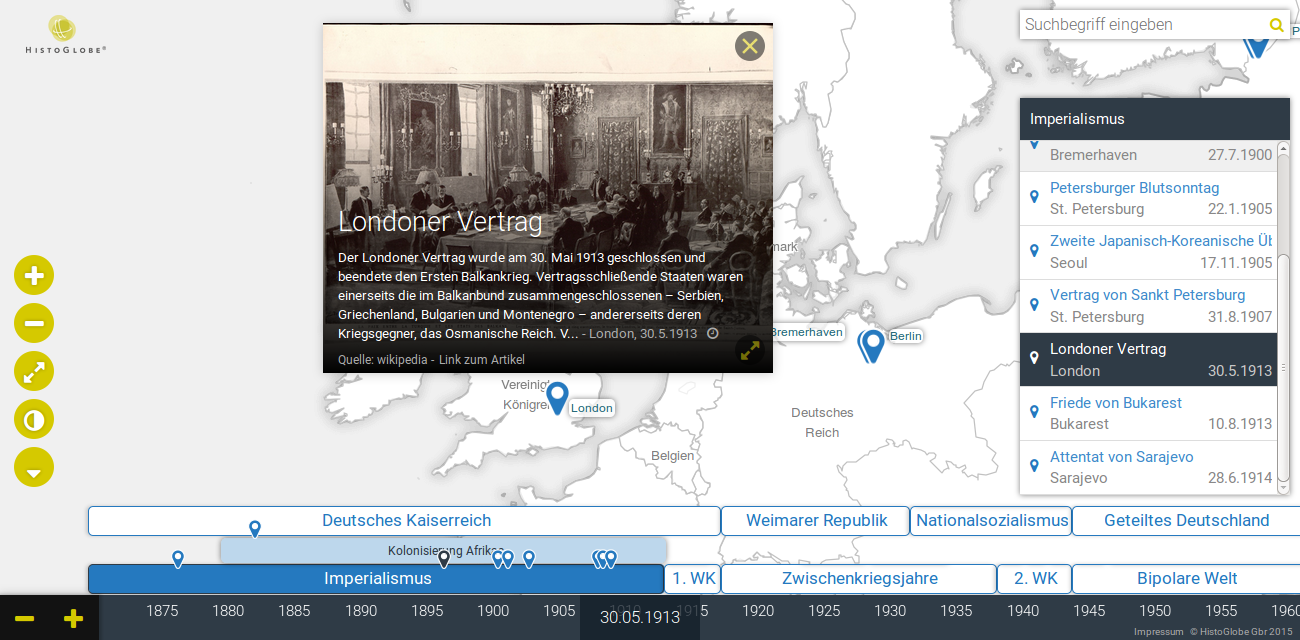
\includegraphics[width=0.9\textwidth]{graphics/hivent_box.png}
  \end{center}
  \caption{Hivent Box displaying information of an historical event with an image}
  \label{fig:hivent_box}
\end{figure}


\paragraph{Small Hivent Box} % (fold)
The small version, as displayed in figure \ref{fig:hivent_box}, is the default representation of our Hivent Boxes. This version is moveable on the map per drag and drop and consists of the same information like the the big Hivent Box, but with a smaller description length.

\paragraph{Big Hivent Box} % (fold)
In figure \ref{fig:hivent_box_big} you can see the big Hivent Box. As mentioned above this version differs only in description length from the small Hivent Box and of course in its size.

\begin{figure}[H]
  \begin{center}
    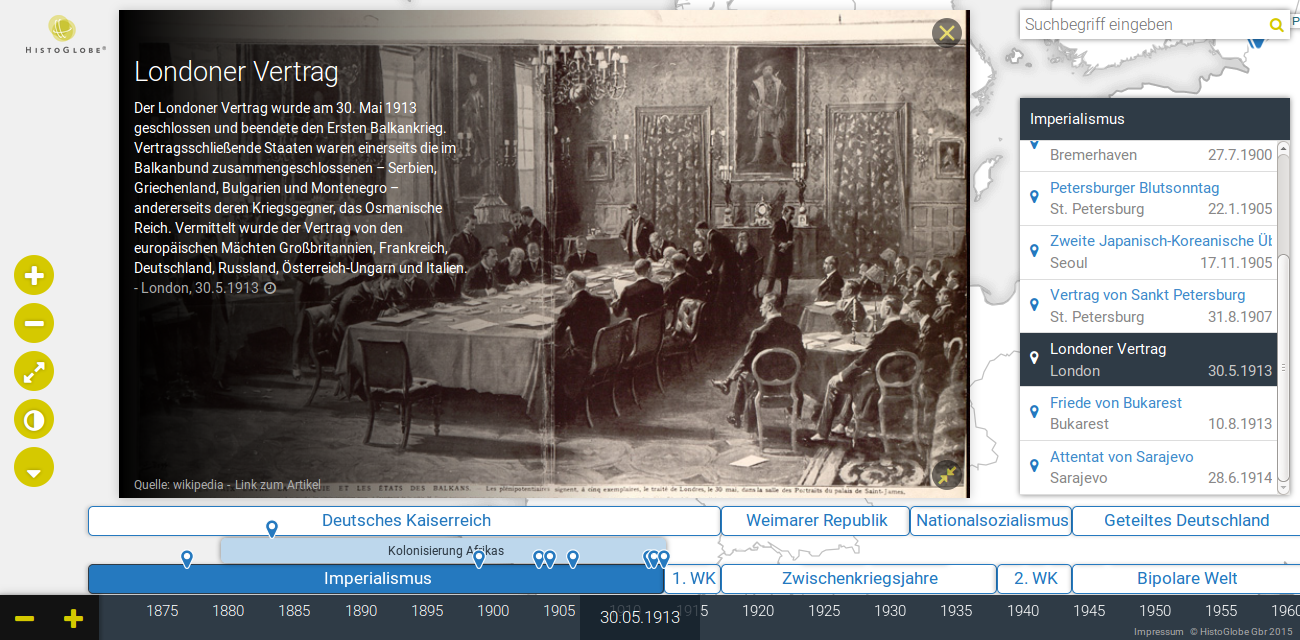
\includegraphics[width=0.9\textwidth]{graphics/hivent_box_big.png}
  \end{center}
  \caption{Big Hivent Box}
  \label{fig:hivent_box_big}
\end{figure}
\label{par:hivent_box_big}

\paragraph{Resize Button - Extend} % (fold)
This button downright is only available in the small version of the Hivent Box and allows the user to switch to the big Hivent Box.
\paragraph{Resize Button - Compress} % (fold)
This button downright is only available in the big version of the Hivent Box and allows the user to switch back to the small Hivent Box.
\paragraph{Multimedia Button} % (fold)
This button on the right is available in both versions of the Hivent Box, the small and the big one, but only if there is existing multimedia content. With this button the user can switch to the multimedia content.

\begin{figure}[H]
  \centering
  \begin{minipage}{0.49\textwidth}
    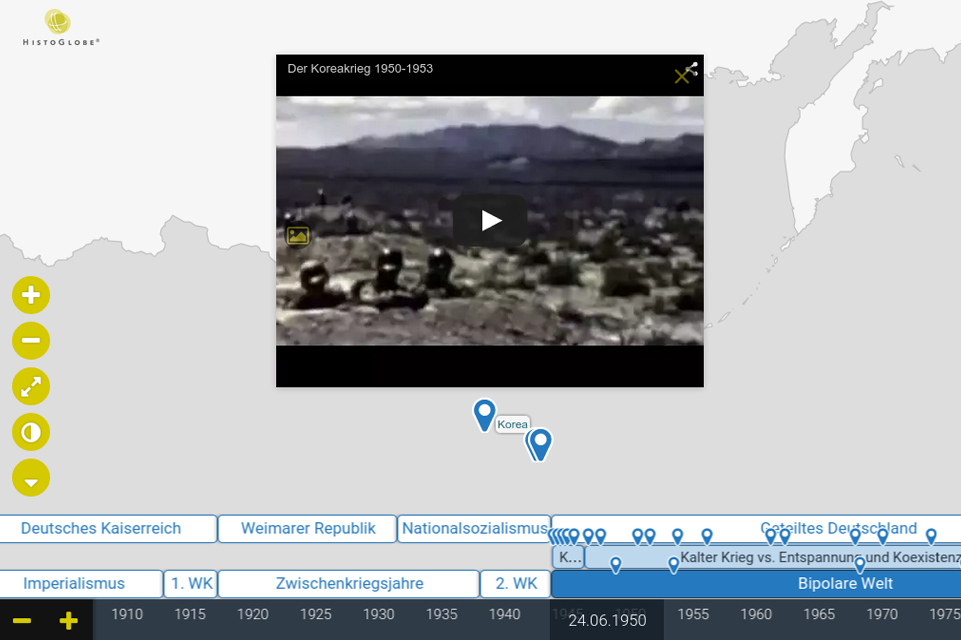
\includegraphics[width=0.95\textwidth]{graphics/smallBox_MM.png}
  \end{minipage}
  \label{fig:multimedia_content_small}
  \begin{minipage}{0.49\textwidth}
    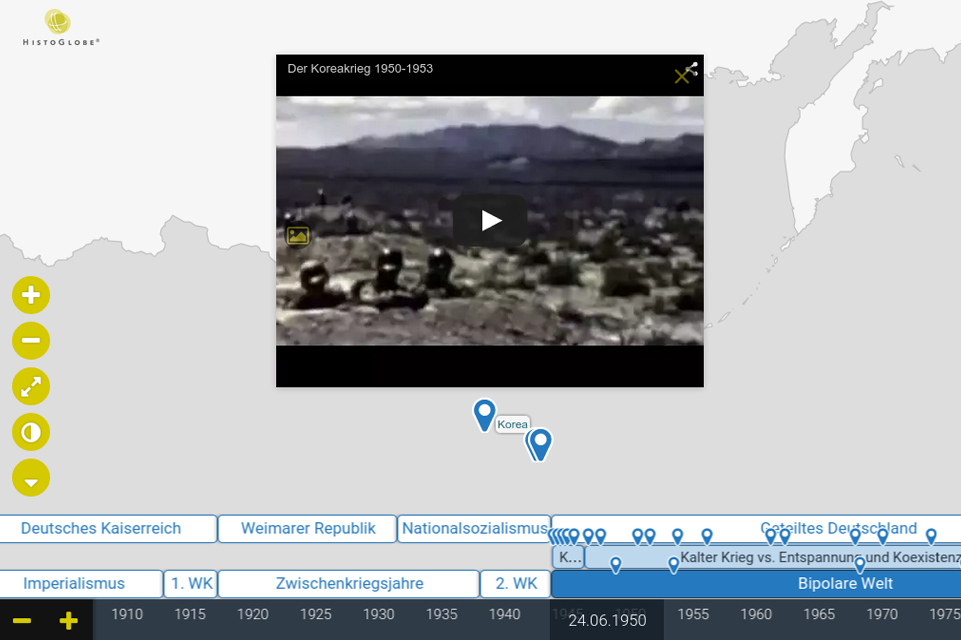
\includegraphics[width=0.95\textwidth]{graphics/bigBox_MM.png}
  \end{minipage}
  \caption{Multimedia content in small and big Hivent Box}
  \label{fig:multimedia_content_small_2}
\end{figure}
\label{par:multimedia_button}

\paragraph{Image Button} % (fold)
This button on the left is only available in the multimedia view of the Hivent Box and allows the user to switch back to normal view.
\paragraph{Close Button} % (fold)
This button in the right upper corner is available in every view and version of the Hivent Box and allows the user to close the box.

% subsection hivent_boxes (end)
